\selectlanguage{english}
\chapter*{Abstract}
\begin{flushleft}
  {\Large\bfseries Separation of Electromyographic Signals According to Their Muscle of Origin\\[0.4cm]}

  \textbf{Author:} Anton Cobian Iregui\\
  \textbf{Supervisor:} Romano Giannetti\\
  \textbf{Collaborating Entity:} Universidad Pontificia Comillas, ICAI
\end{flushleft}
% ── Resumen breve ──────────────────────────────────────────
This Bachelor’s Thesis studies the separation of weak EMG signals mixed with
stronger muscular interference in reinnervated muscle scenarios. ICA, SOBI,
constrained ICA and regression are compared under controlled conditions, showing that recovery depends on mixing, delay and prior information.

\medskip
\noindent\textbf{Keywords:} 
Signal Processing, EMG, Source Separation, Prosthetics
\bigskip

% ── Introducción ───────────────────────────────────────────
\section*{Introduction}

This Bachelor’s Thesis is motivated by a research project developed at the Institute for Research in Technology of Comillas Pontifical University, commonly known as IIT. The project focuses on implantable EMG systems for myoelectric orthoses and bionic reconstruction after severe peripheral nerve injuries. In this context, EMG signals are used to estimate the user’s movement intention and translate it into control commands for prosthetic devices.

However, in reinnervated muscle scenarios, the recorded EMG signal may be affected by attenuation, temporal delays, atypical activation patterns and contamination from donor muscles. This is especially relevant when the target component is weaker than the interfering muscular activity, since the desired information may be masked by stronger sources.

Therefore, this thesis studies whether source separation techniques can help recover weak EMG components from mixed recordings. Rather than reconstruct the exact original waveform, the main goal is to preserve the activation pattern of the target source, which is the most relevant information for EMG control.

\section*{Problem definition}

The specific problem addressed in this work is inspired by the interference that may appear in Vascularized Denervated Muscle Target (VDMT) configurations. In these cases, the target reinnervated muscle can generate a weak EMG signal, while the auxiliary muscle may introduce a stronger contribution into the recorded channel.

\begin{figure}[H]
  \centering
 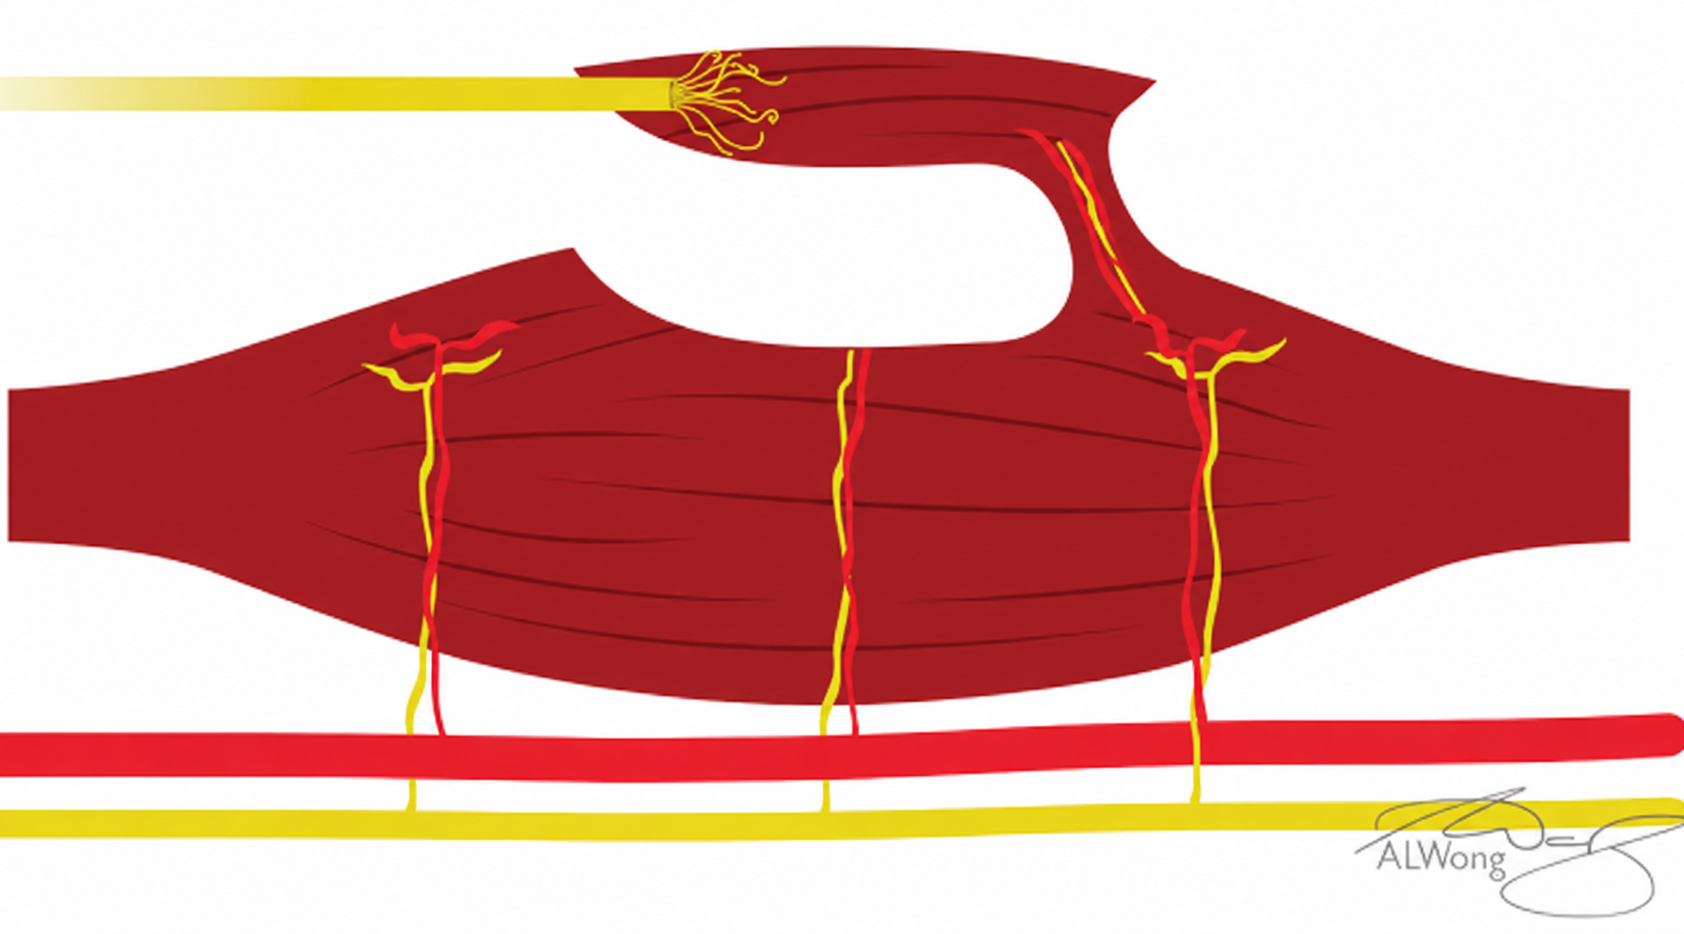
\includegraphics[width=0.8\textwidth]{figuras/VDMT_diagram_modified.png}
  \caption{ Schematic illustration of a VDMT adapted from \cite{tuffaha_vascularized_2020}.}
  \label{fig:abstract_vdmt}
\end{figure}

The separation problem is modeled as a two-source, two-channel system. The target source is expressed as $s_1$, while the stronger interfering source is denoted as $s_2$. Even though several mixture models are considered throughout the thesis to analyze the effect of interference, noise and delay on the general separation process, the IIT case study is modeled using the asymmetric weak-source scenario described in Equation \ref{eq:abstract_model}.

\begin{equation}
    \left\{
\begin{aligned}
c_1(t) &= s_1(t) + \beta s_2(t-\tau) + n_1(t) \\
c_2(t) &= 0.01 s_1(t-\tau) + s_2(t) + n_2(t) 
\end{aligned}
\right.
\label{eq:abstract_model}
\end{equation}
\\
\noindent where $\beta$ represents the interference factor in the weak source, $\tau$ the temporal delay between channels and $n_1(t), n_2(t)$ additive noise with variance $\sigma^2$.

The model represents an asymmetric weak source regime where the target signal is heavily contaminated by the auxiliary muscle while the donor channel contains a minimal contribution from the target source. For this reason, the objective is to estimate the weak source $s_1$ from the observed mixtures and achieve a recovered signal $\hat{s}_1$ that maintains its activation patterns.

\section*{Methodology}

The experimental methodology is structured in several stages. Since specific experimental data from VDMT systems are not yet available, the tests are performed using EMG signals from a dataset of patients with TMR (another muscle reinnervation technique). These signals are used as an experimental basis, along with artificial signals designed to simulate different activation frequencies. The selected signals are then adapted and mixed using the proposed models in order to simulate different levels of interference, noise and delay.

Before applying the separation algorithms, the signals are preprocessed through filtering, channel scaling and whitening. Filtering reduces undesired frequency components, channel scaling improves numerical comparability between channels and whitening prepares the data for the source separation stage.

Several methods are implemented and compared. FastICA is used as the main blind separation algorithm based on non-Gaussianity. SOBI is studied as an alternative method based on temporal correlation. Constrained ICA is introduced to evaluate whether prior information can potentially guide the separation towards the target source. Finally, linear regression is considered as a practical baseline when one channel can be interpreted as an approximate reference of the interfering source.

The outputs are assessed using RMS envelope correlation, temporal correlation and SNR. Among these metrics, RMS envelope correlation is prioritized because EMG-based prosthetic control mainly depends on detecting the activation pattern of the muscle, rather than reconstructing the exact waveform sample by sample. The complete experimental workflow is summarized in Figure \ref{fig:methodoloy_pipeline1}.
\\
\begin{figure}[H]
    \centering
    \makebox[\textwidth][c]{%
    \resizebox{1.20\textwidth}{!}{%
    \begin{tikzpicture}[
        block/.style={
            draw,
            rectangle,
            minimum width=3.0cm,
            minimum height=2cm,
            text width=2.7cm,
            align=center,
            font=\small
        },
        arrow/.style={-{Stealth}, thick},
        label/.style={font=\small, above}
    ]

    \node[block] (sig) {Signal selection\\and \\ conditioning};
    \node[block, right=1.2cm of sig] (mix) {Mixture model};
    \node[block, right=1.2cm of mix] (pre) {Preprocessing};
    \node[block, right=1.2cm of pre] (sep) {Separation\\algorithm};
    \node[block, right=1.2cm of sep] (ass) {Assessment};

    \draw[arrow] (sig.east) -- node[label]{$s_1, s_2$} (mix.west);
    \draw[arrow] (mix.east) -- node[label]{$c_1, c_2$} (pre.west);
    \draw[arrow] (pre.east) -- node[label]{$z_1, z_2$} (sep.west);
    \draw[arrow] (sep.east) -- node[label]{$\hat{s}_1, \hat{s}_2$} (ass.west);

    \end{tikzpicture}
    }%
    }
    \caption{Block diagram of pipeline followed for the experiments in this thesis.}
    \label{fig:methodoloy_pipeline1}
\end{figure}

\section*{Results}

The results show that ICA performs well in ideal or semi-ideal instantaneous mixtures, recovering the sources up to the usual order, sign and scale ambiguities. With additive noise, the temporal correlation of the weak source decreases, although its RMS envelope can still be preserved in some cases.

However, ICA performance worsens when temporal delays are introduced, since an instantaneous separation matrix cannot fully cancel delayed contributions from the dominant source. This mainly affects the recovery of the weak target component, especially when the interfering source has much larger variance.

SOBI does not provide a consistent improvement over ICA for the real EMG signals considered, since their autocorrelation patterns are often too similar. Constrained ICA promises a flexible framework by using prior information, but the binary references tested in this thesis do not show a significant improvement. Delayed regression shows best results only if $c_2$ is a reliable reference of $s_2$ and the delay can be accurately estimated. This suggests that delay-aware or convolutive approaches may directly address the delayed contribution of $s_2$, one of the main limitations of the instantaneous methods studied in this thesis.

\begin{figure}[H]
  \centering
   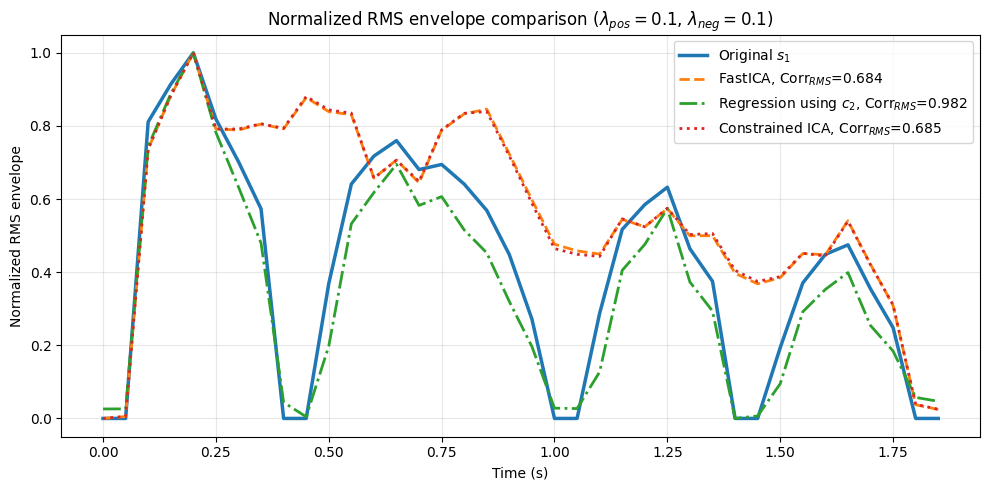
\includegraphics[width=\textwidth]{figuras/comparison_beta_05_tau_5_with_delayed_regression.png}
  \caption{Comparison  of the RMS envelopes recovered by the algorithms. Parameters were set to $\sigma=0.1$, $\beta=0.3$ and $\tau=\qty{5}{ms}$. The delayed regression achieves an almost perfect reconstruction as it removes the delayed interference from $s_2$.}
  \label{fig:abstract_results}
\end{figure}

% ── Conclusiones ───────────────────────────────────────────
\section*{Conclusions}

This thesis shows that source separation methods can be useful for recovering weak EMG components, but their performance depends strongly on the mixing conditions. Specifically, temporal delays, additive noise and source dominance make the recovery of the target signal significantly more difficult.

The main conclusion is that the weak-source problem cannot always be solved reliably with a purely blind and instantaneous approach. When the mixture is close to ideal, standard BSS methods can provide good results, but the IIT scenario introduces additional information that should be exploited whenever possible. In particular, the presence of a reference channel and the estimation of temporal delay become key factors for improving the recovery of the target activation pattern.

Overall, the results suggest that recovering weak EMG activity in some reinnervated muscle scenarios may require more than standard blind separation. Future work should focus on improved delay estimation with convolutive models, meaningful physiological constraints, multichannel EMG signals and validation with real experimental data from the target IIT application.